Let $\vec{x} = \myvec{x\\y}$ be the point. The equation of y-axis is given by
\begin{equation}
    \vec{R} = \lambda \myvec{0\\1}
\end{equation}
$xR$ is perpendicular to y-axis.
\begin{align}
    \implies &(\vec{R} - \vec{x})^\top \vec{R} = 0\\
    \implies &\vec{x}^\top \vec{R} = \norm{\vec{R}}^2\label{1/2/4RelxR}\\
    \implies &\vec{x}^\top \myvec{0\\1}\norm{\vec{R}} = \norm{\vec{R}}^2\\
    \implies &\norm{\vec{R}} = \vec{x}^\top \myvec{0\\1}
\end{align}

Let $\vec{C} = \myvec{2\\1}$. Then
\begin{align}
     xC &= \norm{\vec{x} - \vec{C}}\\
     xR &= \norm{\vec{x} - \vec{R}}
\end{align}

We are given $xR = xC$.  
\begin{align}
    \implies &\norm{\vec{x} - \vec{C}}^2 = \norm{\vec{x} - \vec{R}}^2\\ 
    \implies &\norm{\vec{x}}^2+\norm{\vec{C}}^2-2\vec{x}^\top \vec{C} = \norm{\vec{x}}^2+\norm{\vec{R}}^2-2\vec{x}^\top \vec{R}
\end{align}
Subtracting $\norm{\vec{x}}^2$ on both sides and using \ref{1/2/4RelxR},
\begin{align}
    &\norm{\vec{C}}^2-2\vec{x}^\top \vec{C} = \norm{\vec{R}}^2 - 2\norm{\vec{R}}^2\\
    \implies &2\vec{x}^\top \vec{C} = \norm{\vec{C}}^2+\norm{\vec{R}}^2\\
    \implies &2\vec{C}^\top \vec{x} = \norm{\vec{C}}^2+\myvec{\vec{x}^\top \myvec{0\\1}}^2\\
    \implies &\vec{x}^\top \myvec{0\\1} \myvec{0 & 1} \vec{x} - 2\vec{C}^\top \vec{x} + \norm{\vec{C}}^2 = 0\\
    \implies &\vec{x}^\top \myvec{0&0\\0&1}\vec{x} + 2(-\vec{C})^\top\vec{x} + \norm{\vec{C}}^2 = 0\\
    \implies &\vec{x}^\top \myvec{0&0\\0&1}\vec{x} + 2\myvec{-2&-1}\vec{x} + 5 = 0\\
    \implies &\vec{V} = \myvec{0&0\\0&1},\; \vec{u} = \myvec{-2\\-1},\; f = 5
\end{align}

For obtaining the affine transformation, we use 
\begin{equation}
    \vec{x} = \vec{P}\vec{y}+\vec{c}
\end{equation}

The corresponding eigenvalues of $\vec{V}$ are
\begin{align}
    \lambda_1 = 0,\; \lambda_2 = 1\\
    \implies \vec{D} = \myvec{0&0\\0&1}
\end{align}

The corresponding eigenvectors are
\begin{align}
    &\vec{p}_1 = \myvec{1\\0},\; \vec{p}_2 = \myvec{0\\1}\\
    \implies &\vec{P} = \myvec{\vec{p}_1 & \vec{p}_2} = \myvec{1&0\\0&1}
\end{align}

Since $\abs{\vec{V}} = 0$,
\begin{align}
    \myvec{\vec{u}^\top+\eta \vec{p}_1^\top\\\vec{V}}\vec{c} &= \myvec{-f\\\eta \vec{p}_1-\vec{u}}\\
    \eta &= \vec{u}^\top \vec{p}_1\\
    \implies \eta &= -2\\
    \implies \myvec{-4&-1\\0&0\\0&1}\vec{c} &= \myvec{-5\\0\\1}\\
    \implies \vec{c} &= \myvec{1\\1}
\end{align}

Therefore, the locus of $\vec{x}$ is given by
\begin{align}
    \vec{y}^\top \myvec{0&0\\0&1}\vec{y} = 4\myvec{1&0}\vec{y}
\end{align}

\begin{figure}[h]
    \centering
    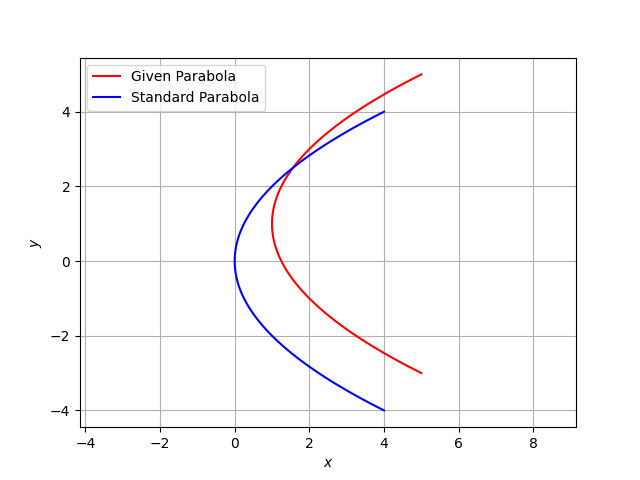
\includegraphics[width=\columnwidth]{solutions/1/2/4/figures/figure.png}
    \caption{Plot of the locus}
    \label{1/2/4fig}
\end{figure}
